\documentclass[a4paper,10pt,twocolumn]{article}
\\usepackage[T1]{fontenc}
\usepackage[english]{babel}
\usepackage[a4paper,
            top=1.25cm, bottom=4.2cm, left=2.6cm, right=2.6cm,
            includehead, headheight=2.83cm, headsep=0.15cm]{geometry}
\usepackage[scaled]{helvet}            % Arial substitute
\usepackage{graphicx}                  % \includegraphics
\usepackage{fancyhdr}                  % logo in the page header
\usepackage{caption}                   % "Picture N: ..." captions
\usepackage{titlesec}                  % 13 pt bold centred headings
\usepackage[authoryear,round]{natbib}  % \citet{key} -> "Helsgaun (2017)"
\usepackage[hidelinks]{hyperref}       % keep last

% --- Arial substitute as the default family
\renewcommand{\familydefault}{\sfdefault}

% --- two columns, 0.8 cm apart, no separating rule (as in the template)
\setlength{\columnsep}{0.8cm}
\setlength{\columnseprule}{0pt}

% --- bibliography: author-year style, entries not spaced apart
\bibliographystyle{plainnat}
\setlength{\bibsep}{0pt plus 1pt}
% The template's margins are generous (4.2 cm at the bottom) and this
% abstract carries two figures where the template carries one, so the
% reference list is set one point down to hold the two-page limit.
\renewcommand{\bibfont}{\fontsize{9}{11}\selectfont}

% --- header: logo top-left on every page, no rule, no page number
\pagestyle{fancy}
\fancyhf{}
\renewcommand{\headrulewidth}{0pt}
% The logo was extracted from template.doc and cropped to its ink bounding
% box, so 3.2 cm here matches the size it has in the Word template.
\fancyhead[L]{
\includegraphics[width=3.2cm]{Figures/siicusp34_logo.png}}

% --- section headings: 13 pt bold, centred, 6 pt above and below
\titleformat{\section}
  {\centering\fontsize{13}{15.6}\selectfont\bfseries}{}{0pt}{}
\titlespacing*{\section}{0pt}{6pt}{6pt}

% --- captions: 9 pt, centred, "Picture N: ..." with no bold
\DeclareCaptionFont{ninept}{\fontsize{9}{11}\selectfont}
\captionsetup{labelsep=colon, font=ninept,
              labelfont={}, textfont={}, justification=centering,
              skip=6pt}
\captionsetup[figure]{name=Picture}

% --- body: no paragraph indent, no extra space between paragraphs
\setlength{\parindent}{0pt}
\setlength{\parskip}{0pt}

% --- tighter float separation, so the abstract holds to two pages
\setlength{\textfloatsep}{10pt plus 2pt minus 2pt}
\setlength{\floatsep}{10pt plus 2pt minus 2pt}
\setlength{\intextsep}{10pt plus 2pt minus 2pt}
\setlength{\dbltextfloatsep}{10pt plus 2pt minus 2pt}
\setlength{\dblfloatsep}{10pt plus 2pt minus 2pt}
% let a page carry more float and less mandatory text, so no float-only page
\renewcommand{\topfraction}{0.92}
\renewcommand{\bottomfraction}{0.85}
\renewcommand{\textfraction}{0.06}
\renewcommand{\floatpagefraction}{0.88}
% The two charts are figure* (full width), and full-width floats obey a
% separate set of parameters. Left at their defaults, the pair fills ~54%
% of the text height, which clears the 0.5 default of \dblfloatpagefraction
% and gets them banished to a float-only page. Raising both keeps them at
% the top of a normal page with the running text underneath.
\renewcommand{\dbltopfraction}{0.9}
\renewcommand{\dblfloatpagefraction}{0.9}
\raggedbottom

% --- title-block line: 13 pt, 12 pt of space below (as in the template)
\newcommand{\siicline}[1]{%
  {\centering\fontsize{13}{15.6}\selectfont #1\par}\vspace{12pt}}

\begin{document}

% =====================================================================
%  TITLE BLOCK — the template's first section, spanning the full width
%  above the two columns.
%  TODO: preencher os campos marcados abaixo antes de submeter.
% =====================================================================
\twocolumn[%
\vspace*{6pt}

\siicline{\bfseries Benchmarking Metaheuristic and Learning-Based Solvers
for the Traveling Salesman Problem in a Last-Mile Delivery Application}

\siicline{\bfseries Rafael Maziero Araujo}

\siicline{\bfseries Prof. Dr. Marlon Fernandes de Souza}

% TODO: unidade e universidade
% (sem \bfseries de propósito: no template esta linha é a única do bloco
%  de título em peso normal)
\siicline{Escola Superior de Agricultura "Luiz de Queiroz" | Universidade de São Paulo (USP)}

{\centering\fontsize{10}{12}\selectfont
 rafamazaraujo@usp.br\par}
\vspace{12pt}
]

% =====================================================================
\section{Objectives}

RouTrip is an open-source application that turns a delivery order sheet into an
optimized last-mile route. Addresses are read by optical character recognition,
interpreted and corrected by generative artificial intelligence models, and sent
to the OpenRouteService API, which returns an asymmetric from-to distance
matrix. The solver embedded in this pipeline must return a short route, but it
must return it fast enough for interactive use on ordinary hardware. This work
benchmarks five solvers of distinct natures over instances ranging from 5 to 100
stops, and selects the default solver from the joint analysis of quality and
runtime, rather than from quality alone.

\section{Materials and Methods}

The asymmetric matrix produced by the routing API is converted into an
equivalent symmetric instance by the transformation of \citet{jonker1983},
which makes the whole body of symmetric TSP solvers available to the
application. Five algorithms of distinct families were compared: the
Lin--Kernighan--Helsgaun solver (LKH3) of \citet{helsgaun2017}, the Iterated
Local Search (ILS) of \citet{lourenco2003}, the Adaptive Large Neighborhood
Search (ALNS) of \citet{ropke2006}, the Hybrid Genetic Search (HGS) of
\citet{vidal2022}, and a Graph Neural Network (GNN) trained to construct tours
following \citet{kool2019}.

The benchmark covers five instance sizes --- 5, 10, 20, 50 and 100 cities ---
with 20 random seeds each, totalling 100 runs per algorithm, all implemented in
Python 3.11 and executed on the same machine. Three metrics were recorded per
run: the optimality gap, that is, how much the tour cost exceeds the best cost
found for that instance by any solver; the runtime in seconds; and the win rate,
the percentage of runs reaching that best cost.
% TODO: descrever o hardware e o critério de parada de cada metaheurística.

\section{Results}

Up to 20 cities the solvers are essentially indistinguishable in quality, with
the single exception of ALNS, which already loses 0.887\% at 10 cities and
1.996\% at 20 (Picture~\ref{fig:gap_time}a). Differences appear only as the instances grow: at
100 cities ALNS reaches a mean gap of 4.251\%, the GNN 1.336\% and ILS 0.258\%,
while HGS and LKH3 remain at 0.000\%. Runtime separates them far more sharply
(Picture~\ref{fig:gap_time}b): LKH3 scales almost flat, from 0.061~s at 5 cities
to 0.135~s at 100, whereas ALNS climbs to 27.945~s. At 100 cities the GNN takes
12.030~s, ILS 8.124~s and HGS 7.432~s.

% figure* spans both columns: these are two-panel charts and would be
% unreadable at the 7.5 cm width of a single column.
\begin{figure*}[!tbp]
    \centering
    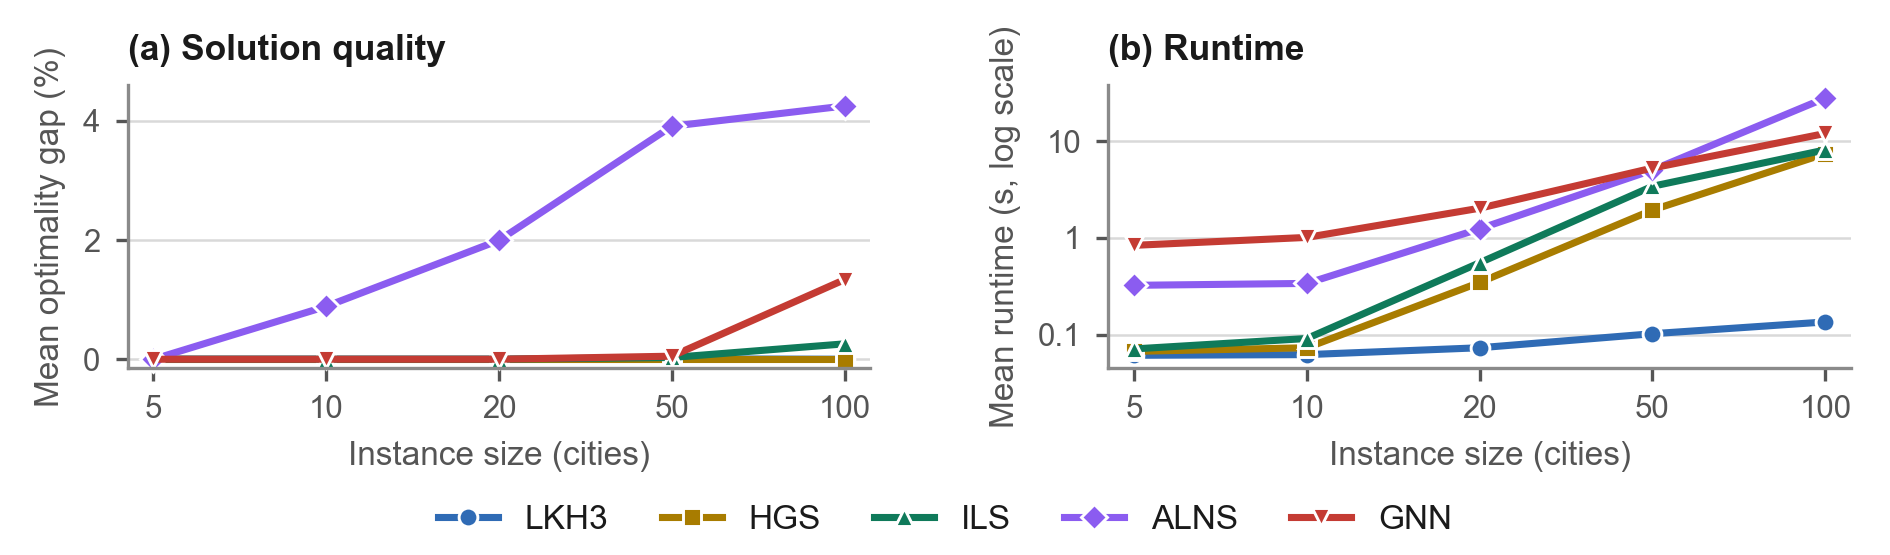
\includegraphics[width=\textwidth]{Figures/fig1_gap_time.png}
    \caption{Mean optimality gap (a) and mean runtime (b) of the five solvers
    across instance sizes, over 20 seeds per size.}
    \label{fig:gap_time}
\end{figure*}

Combining both axes on the largest instance (Picture~\ref{fig:tradeoff}a), LKH3 is the only
non-dominated solver: it matches the best mean gap while being roughly 55 times
faster than HGS, the closest competitor in quality. The win rate (Picture~\ref{fig:tradeoff}b)
shows that the quality tie between the two is not exact --- HGS returned the
best tour in 100\% of the runs against 99\% for LKH3 --- but the remaining
difference is smaller than the third decimal place of the mean gap. ILS reached
the best tour in 89\% of the runs, the GNN in 79\% and ALNS in only 49\%.

\begin{figure*}[!tbp]
    \centering
    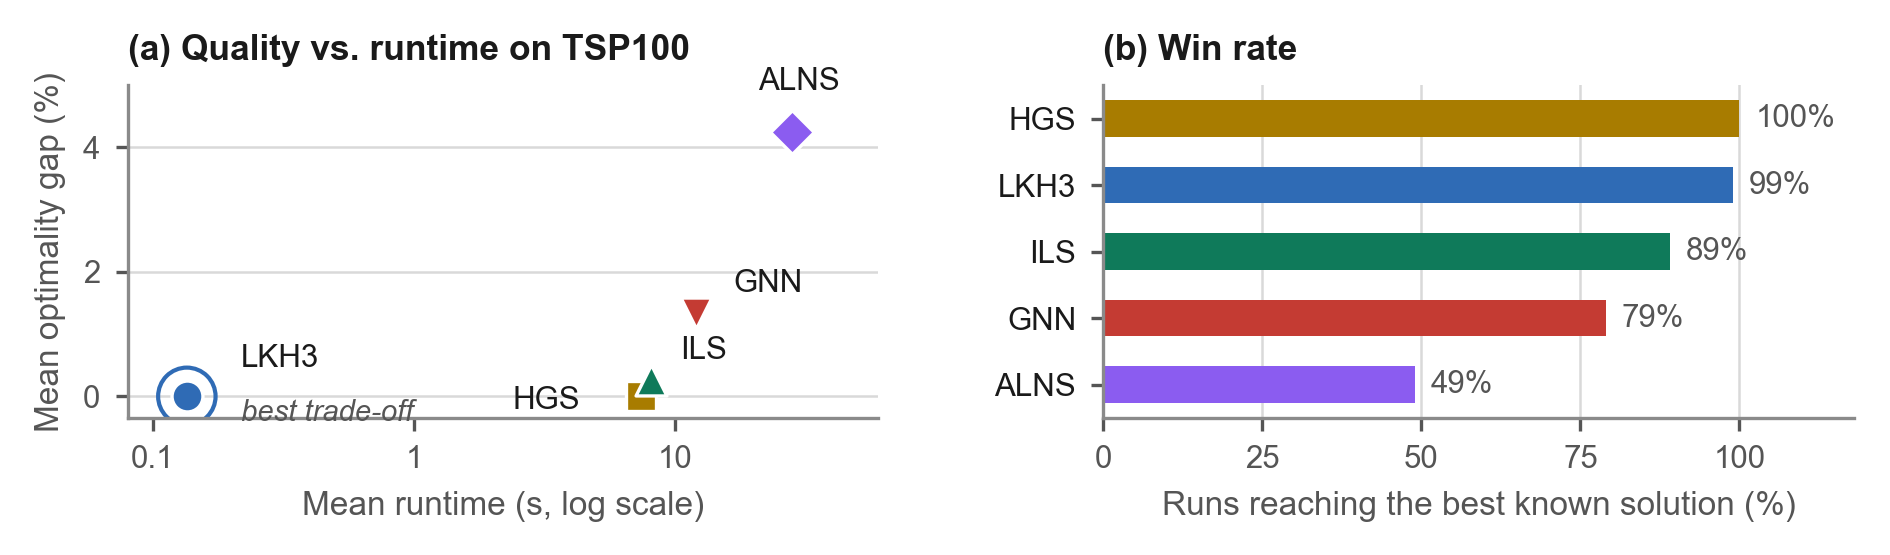
\includegraphics[width=\textwidth]{Figures/fig2_tradeoff_winrate.png}
    \caption{(a) Quality versus runtime on the 100-city instances, where LKH3 is
    the only non-dominated solver. (b) Percentage of runs in which each solver
    reached the best known tour, over all instance sizes.}
    \label{fig:tradeoff}
\end{figure*}

\section{Conclusions}

For the range of instance sizes a last-mile delivery route actually reaches,
LKH3 is the default solver of RouTrip: it is statistically as accurate as the
best alternative while running in a fraction of a second, which is the only
behaviour compatible with an interactive application. HGS remains the reference
for solution quality and is the natural fallback whenever runtime is
irrelevant. ALNS was the weakest solver on both axes and was discarded. The GNN
is promising but not yet competitive at these scales: its inference cost does
not pay off against classical heuristics on instances of a hundred stops.

The authors declare no conflict of interest.

Rafael M. Araujo designed and implemented the benchmark and analysed the
results. % TODO: descrever a contribuição dos colaboradores e do orientador,
% ajustando a frase abaixo.
The supervisor contributed to the study design and to the final revision. All
authors approved the final version of the abstract.

% TODO: informar a bolsa acadêmica, se houver (ex.: bolsa PUB/USP ou de agência
% de fomento). Se não houver, apagar a linha abaixo.
This research was carried out with the support of an undergraduate research
scholarship.

% As referências saem de bibtex/siicusp2026.bib; o próprio \bibliography
% emite o título "References" com a formatação de \section definida acima.
\bibliography{bibtex/siicusp2026}

\end{document}
